\documentclass[12pt]{article}
\usepackage[margin = 1in]{geometry}
\usepackage{inputenc}
\parindent 0px
\usepackage{float}
\usepackage{amsfonts, amsmath, amssymb}
\usepackage{hyperref}
\usepackage{graphicx}
\bibliographystyle{plain}
\usepackage{xcolor}
\pagecolor{white}
\usepackage{tikz}
\usetikzlibrary{shapes, arrows.meta, positioning}

\title{Software System Laboratory\\Project Proposal}
\author{Team name: \large KaryM}
\date{}

\begin{document}
\maketitle
\section*{Team members}
\begin{itemize}
\item Nithin Sabu (\textbf{210010032})
\item Suyash Gaurav (\textbf{210010054})
\item Himanshu Kumar (\textbf{210010019})
\item Poorvasha Dhananjay Chauhan (\textbf{210010040})
\item Vishal Gandluri (\textbf{210010017})
\end{itemize}
\section*{Our proposal}
\begin{itemize}
    \item The fundamental idea of the project is to connect unskilled/skilled labour or those who can provide labour (i.e. contractor) with those who are in need of it.
    \item There are mainly three parties involved here: customers, labourers and contractors. This model connects the nearest possible labour or labour supplier to the customer.
\end{itemize}
\section*{Who are our Users:}
\begin{itemize}
\item The customers who need labour, can register through the website using either their email or phone number.
\item The labourer can either connect directly, if possible, or through a contractor whom he is affiliated with. Both skilled and unskilled labourers are welcome to register on our website and search for appropriate jobs.
\item The contractor who have labours working under him and can provide labours when demnaded.
\end{itemize}

\section*{Working principle}
\begin{itemize}
\item The website will connect the labourer with the client in two ways: directly or through the contractors.
\item The labourers who are looking for work or a contractor who is willing to provide work can join our network.
We will take the details and location of the labourer and contractor and store it in the backend database.
\item When a customer submits a work request, the request is enqueued and labourers and contractors will be notified regarding the same. Once the labourer/contractor accepts the deal, the 
customer is  connected to  the labourer/contractor. Both the users may contact each other. The labourer will then proceed to the workplace to complete the necessary work.
\item Additionally, labourers have the choice to add their profiles in which they can mention their skills to the website so that customers can view them. 

\end{itemize}

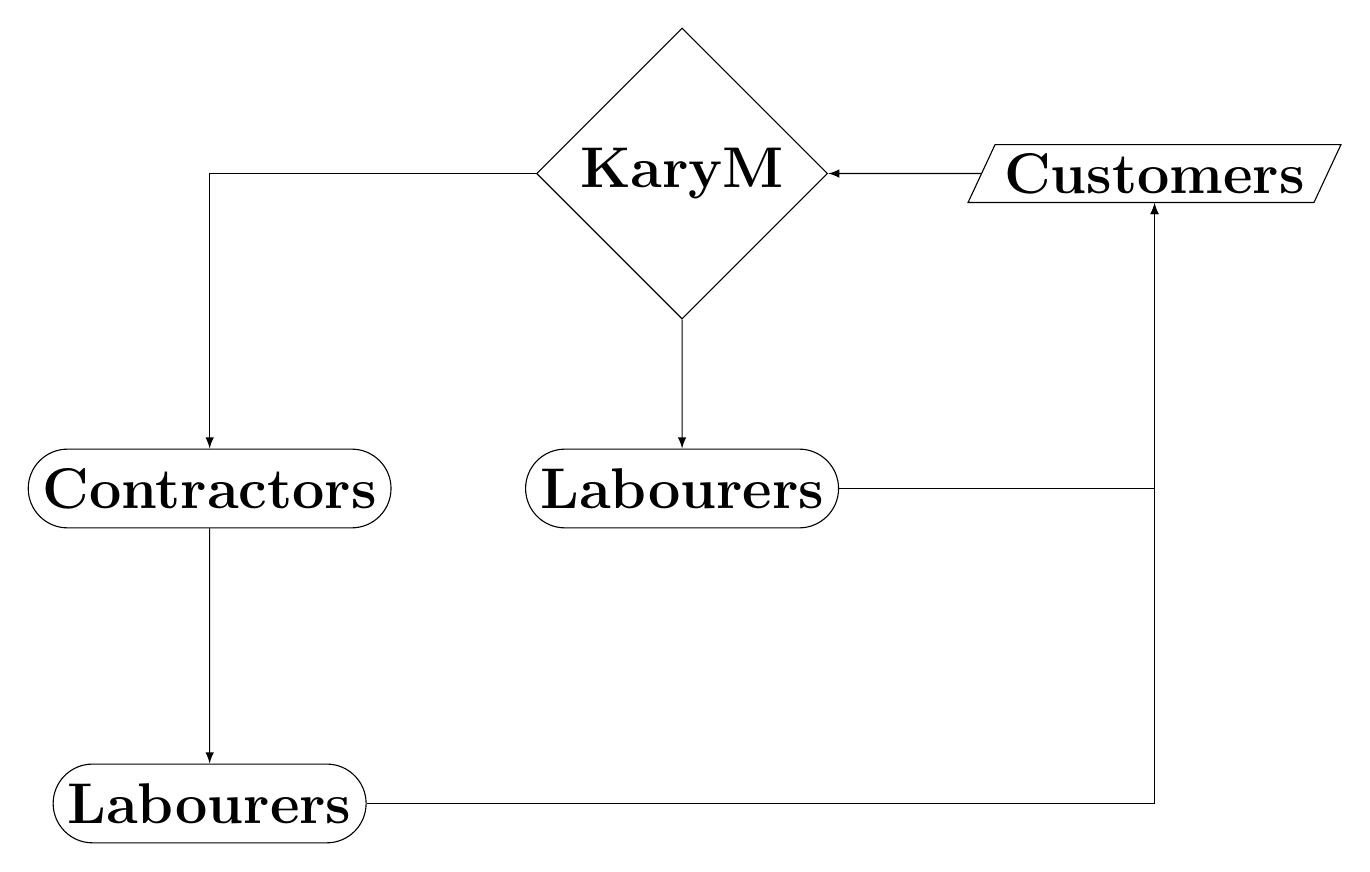
\begin{tikzpicture}

\node[diamond,draw] at (6,0) (block1) {{\huge \textbf{KaryM}}};

\node[draw,
    rounded rectangle, 
    minimum width=2.5cm,minimum height=1cm] at (0,-4) (block2) {{\huge \textbf{Contractors}}};
    
\node[draw,
    rounded rectangle, 
    minimum width=2.5cm,minimum height=1cm] at (0,-8) (block3)  {{\huge \textbf{Labourers}}};
    
\node[draw,
    rounded rectangle, 
    minimum width=2.5cm,minimum height=1cm] at (6,-4) (block4) {{\huge \textbf{Labourers}}};
    
\node[draw,
    trapezium,
    trapezium left angle = 65,
    trapezium right angle = 115,
    trapezium stretches] at (12,0)  (block5) {{\huge \textbf{Customers}}};
    
\draw[-latex] (block1) -| (block2);
\draw[-latex] (block3) -| (block5);   
\draw[-latex] (block4) -| (block5);   
\draw[-latex] (block1) edge (block4) 
              (block2) edge (block3) 
              (block5) edge (block1);
    
\end{tikzpicture}
\pagebreak


\section*{Website Structure}
\begin{itemize}
\item The home page is the first page, from which both customers and labourers/contractors are forwarded to their respective login pages.
\item Customers and labourers/contractors can login using their sign in page if they are already registered users, if not they can create a new account.
\item A labourer or contractor can view customer requests based on the skill they can provide after signing up. They can then decide which request best suits them. If they want to update their profile, they can visit their profile page.
\item Customers who log in are presented with profiles of the labourers and contractors so they can get in touch with them and then they can submit a work request. Following that, their project proposal will be shown to the labourer/contractor.
\end{itemize}


\section*{Practical applications and need for this}
\begin{itemize}
\item The problem this project tries to tackle is unorganised and non-uniform distribution of labour. Due to the existing recruitment structure, there is a chance that there will be a labour shortage on one side and a need for the same on the other.
\item The project's aim is to make the recruitment process more efficient by increasing the odds of both the customer finding the required labour and the labourer finding the needed work.
\end{itemize}

\section*{PROGRAMMING LANGUAGES USED}
\textbf{Frontend}
\begin{itemize}
    \item HTML - For giving the structure to the web-page.
    \item CSS - For designing part.
\end{itemize}
\textbf{Backend}
\begin{itemize}
    \item PHP - To create dynamic content and to interact with databases.
    \item MYSQL - For Storing databases.
\end{itemize}
\end{document}



 





